\documentclass[border=10pt]{standalone}
\usepackage{tikz}\usepackage{amsmath}\usetikzlibrary{calc,arrows.meta}
\begin{document}
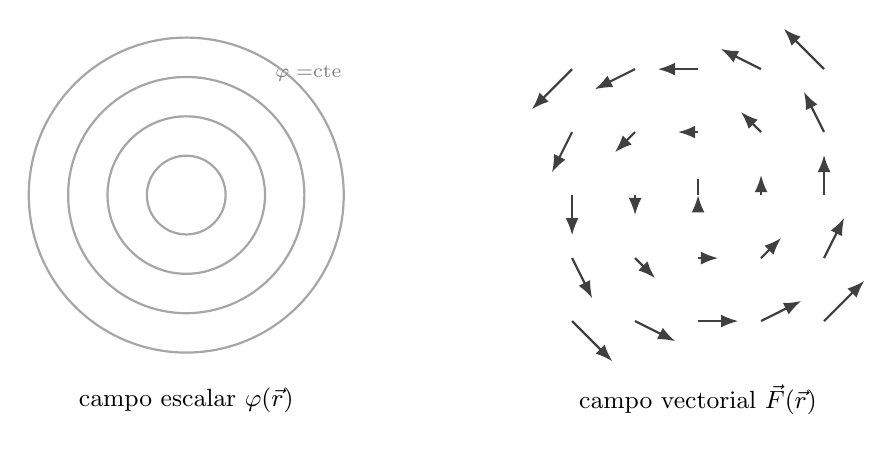
\begin{tikzpicture}[line width=0.8pt,>={Latex[length=2.2mm]}]
  % escalar: curvas de nivel
  \foreach \r in {0.5,1.0,1.5,2.0} \draw[gray!70] (0,0) circle(\r);
  \node at (0,-2.6){\small campo escalar $\varphi(\vec r)$};
  \node[gray] at (1.55,1.55){\scriptsize $\varphi=$cte};
  % vectorial: rejilla de flechas (campo rotacional de ejemplo)
  \begin{scope}[xshift=6.5cm]
    \foreach \x in {-1.6,-0.8,0,0.8,1.6} \foreach \y in {-1.6,-0.8,0,0.8,1.6}{
      \pgfmathsetmacro{\ux}{-\y*0.32}\pgfmathsetmacro{\uy}{\x*0.32}
      \draw[->,black!75] (\x,\y)--++(\ux,\uy);
    }
    \node at (0,-2.6){\small campo vectorial $\vec F(\vec r)$};
  \end{scope}
\end{tikzpicture}
\end{document}
